\documentclass[british,titlepage,twoside]{ntnuthesis}

\title{Paving the Way for Enhanced Situational Awareness in the Maritime Domain: 
Designing and Ensembling a Sensor Rig for Multi-Sensor Data Set Acquisition}
\shorttitle{Sensor Rig for Multi-Sensor Data Set Acquisition}
\author{Emil Martens}
\shortauthor{Emil Martens}
\date{Spring 2023}
\addbibresource{thesis.bib}


% --------------------
% ----- Commands -----
% --------------------
\newcommand{\code}[1]{\hspace{-.3em}\mintinline{text}{#1}\hspace{-.3em}\xspace}
\newcommand{\todo}{\textcolor{red}{Todo}\xspace}
\newcommand{\review}{}
% \newcommand{\review}{\textcolor{green}{Draft Complete}\\}
\newcommand{\done}{}
% \newcommand{\done}{\textcolor{olive}{Done}\\}
\makeglossaries

\setabbreviationstyle[acronym]{long-postshort-user}
\glssetcategoryattribute{acronym}{nohyperfirst}{true}
\setabbreviationstyle{short-nolong}

\newglossaryentry{asyncio}{name=thing,description={A Python library for asynchronous code using coroutines, event loops, and tasks.}}
% --------------------
% ----- Acronyms -----
% --------------------

\newacronym{nvs}{NVS}{Novel View Synthesis}
\newacronym{mlp}{MLP}{Multi-Layer Perceptron}
\newacronym{nerf}{NeRF}{Neural Radiance Field}
\newacronym{rt}{RT}{Ray Tracing}
\newacronym{bvh}{BVH}{Bounding Volume Hierarchy}

% \glsaddall
% \glsunset{cpu}
% \glsunset{gpu}
% \glsunset{lla}
% --------------------
% ----- Shortcuts ----
% --------------------


\newcommand{\nvidia}{NVIDIA\xspace}

\newcommand{\jetson}{\gls{jetson}\xspace}
\newcommand{\sr}{Sensor Rig\xspace}
\newcommand{\jx}{Xavier\xspace}
\newcommand{\jo}{Orin\xspace}
\newcommand{\gs}{Gstreamer\xspace}
\newcommand{\cam}{Triton Polarizin Camera\xspace}
\newcommand{\cams}{Triton Polarizin Cameras\xspace}
\newcommand{\lucid}{Lucid Vision\xspace}
\newcommand{\preproject}{Pre-Project\xspace}
\newcommand{\master}{Master's\xspace}
\newcommand{\py}{Python\xspace}
\newcommand{\cpu}{\gls{gpu}\xspace}
\newcommand{\gpu}{\gls{cpu}\xspace}
\newcommand{\gui}{GUI\xspace}
\newcommand{\guif}{\gls{gui} framework\xspace}
\newcommand{\srgui}{\sr \gls{gui}\xspace}
 
% \oneside
% 
\emergencystretch=1em
% \includeonly{chapters/10_intro/__include__}
% \includeonly{chapters/30_debayer_in_cuda/__include__}

\begin{document}
% \includepdf{chapters/10_intro/frontpage.pdf}
\tableofcontents


\section{Paper Summary}

\begin{figure*}
    \centering
    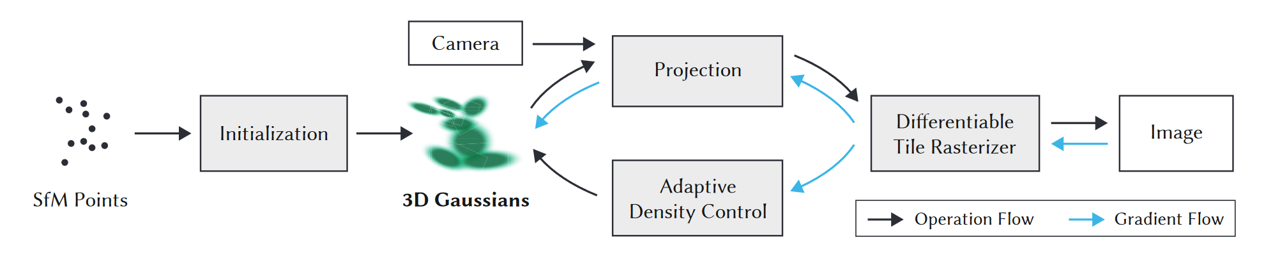
\includegraphics[width=\textwidth]{images/pipeline.png}
    \caption{The Gaussian splatting pipeline presented in the paper \cite[Fig. 2]{kerbl3DGaussianSplatting2023}.}
\end{figure*}


\subsection{Representation}
The core idea of the paper is to represent the scene as a set of Gaussians.
Each Gaussian is defined by its position $\bm{p}$, its covariance matrix $\bm{\Sigma}$, its color $\bm{c}$ and its opacity $\alpha$.

As the covariance has to be symmetric and positive definite, it is defined as
\begin{align}
    \bm{\Sigma} = \bm{R} \bm{S} \bm{S}^T \bm{R}^T,
\end{align}
where $\bm{R}$ is a rotation matrix stored as a quaternion $\bm{q}$ and $\bm{S}$ is a diagonal matrix containing the standard deviation of the Gaussian along each axis stored as a vector $\bm{s}$
To ensure that the covariance is positive definite, the diagonal elements of $\bm{S}$ are passed through a sigmoid function.
The quaternion $\bm{q}$ is normalized to ensure a proper rotation matrix.

% Similarly to other \cite{yuPlenoxelsRadianceFields2021a}\cite{mullerInstantNeuralGraphics2022}


\subsubsection{Spherical Harmonics}
\begin{figure}
    \centering
    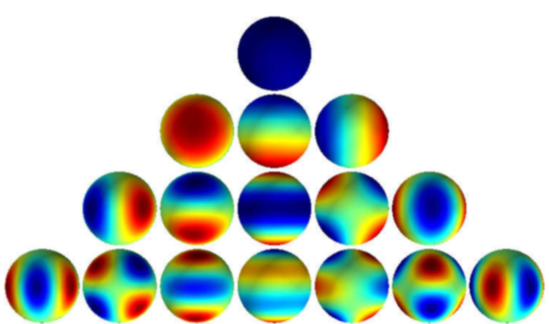
\includegraphics[width=\linewidth]{images/spherical_harmonics.png}
    \caption{Visualization of the spherical harmonics used to represent the view-dependent color of each Gaussian \cite[Fig. 3]{kerbl3DGaussianSplatting2023}.}
\end{figure}

\subsubsection{Camera Projection}

\subsection{Rasterization Pipeline}
\begin{figure}
    \centering
    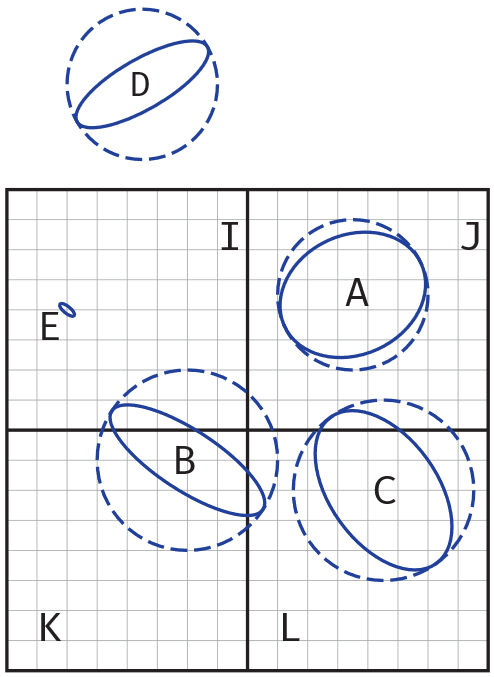
\includegraphics[width=0.6\linewidth]{images/rendering.png}
    \caption{Visualization of how Gaussian splats are rendered using multiple independent blocks.}
\end{figure}
\label{sec:rasterization}

\subsection{Densification}
\begin{figure}
    \centering
    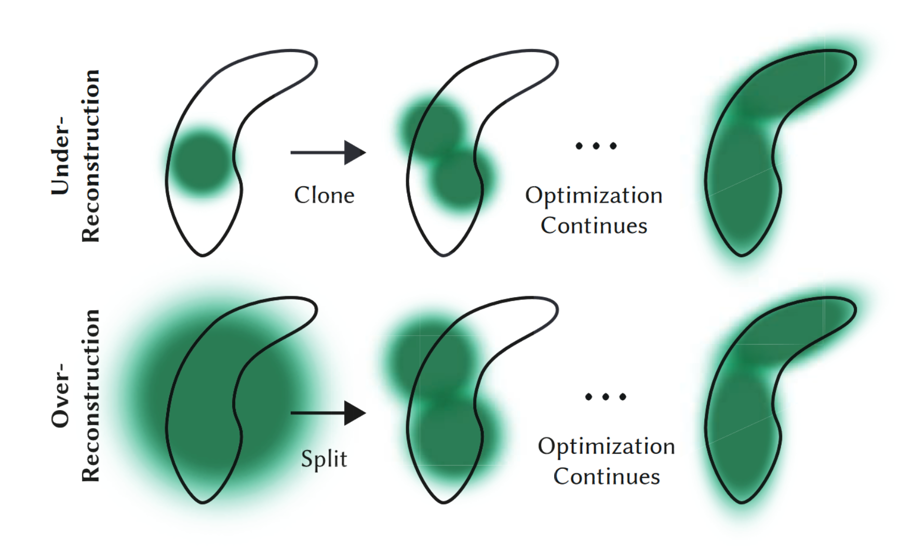
\includegraphics[width=\linewidth]{images/densification.png}
    \caption{The adaptive Gaussian densification scheme presented in the paper \cite[Fig. 4]{kerbl3DGaussianSplatting2023}.}
\end{figure}

% \listoffigures
% \listoftables
% \lstlistoflistings 
\pagebreak

% \input{chapters/__include__.tex}

\newglossarystyle{mystyle}{\glossarystyle{long}\renewenvironment{theglossary}%
    {\footnotesize \begin{longtable}{p{3cm}p{\glsdescwidth}}}{\end{longtable}}%
}
\printglossary[style=mystyle,type=\acronymtype]
\printglossary[style=mystyle]
\AtNextBibliography{\footnotesize}
\printbibliography

% \chapter{Additional resources}
\label{chap:additional_resources}
% \include{appendices/index_table.tex}
% \include{appendices/forum_posts.tex}
% \include{appendices/compilation.tex}
% \include{appendices/curaconfig.tex}


\end{document}
